\chapter{Komponentenauswahl und Schaltungsdesign}
\section{H-Brücke}
Zur Ansteuerung des Aktors wird eine H-Brücke verwendet. 
Als Halbbrücken dienen zwei BTN8982 (Datenblatt in Anhang !!!) mit jeweils einem p-channel highside MOSFET und einem n-channel lowside MOSFET mit bereits integrierten Schutzmechanismen wie Abschaltung bei zu geringer Spannung oder Übertemperatur beinhalten.  Die Halbbrücken sind für Ströme bis zu 55 Ampere sowie Spannungen bis zu 40 Volt ausgelegt und sind temperaturbeständig bis 150° Celsius. Das Blockdiagramm dieser Halbbrücken ist in nachstehender Abbildung dargestellt.
\begin{figure}[h]
	\centering
		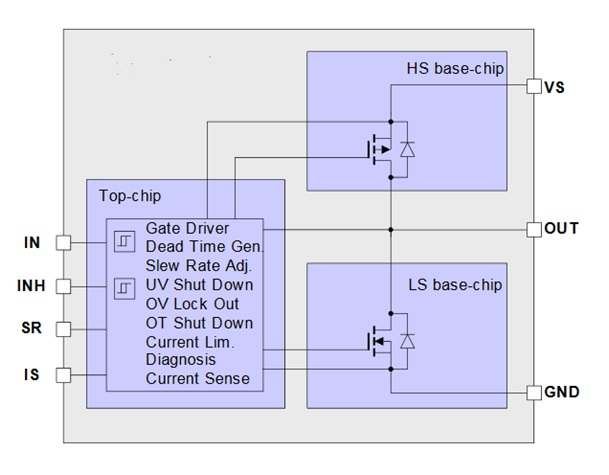
\includegraphics{Bilder/Blockdiagramm Halbbruecken.jpg}
	\caption{Blockdiagramm Halbbrücken}
	\label{fig:Blockdiagramm Halbbruecken}
\end{figure}
In dem Blockdiagramm sind bereits die PINs der Halbbrücken zu erkennen. Diese sollen nun in Tabelle \ref{tab:Pinverteilung} nochmal aufgezählt und ihre Funktionen erklärt werden. 

\begin{table}[h]
	\centering
		\begin{tabular}{l|p{2,5cm}|p{8cm}|p{3cm}}
			\textbf{Pin Nummer} & \textbf{Bezeichnung} & \textbf{Erläuterung} & \textbf{Anschluss an} \\ \hline
			1 & GND (Ground) & Erdung & Ground MCU \\
			2 & IN (Input) & definiert die Schalterstellung (1 = High Switch Mode; 0 = Low Switch Mode) & O-Pin MCU \\
			3 & INH (Inhibit) & 1: Betriebsmodus, 0: Schlafmodus & O-Pin MCU \\
			4, 8 & OUT (Output) & Ausgang der Brückenschaltung & Aktor \\
			5 & SR (Slew Rate) & Einstellen der Steigung der Spannungsantwort & kurzgeschlossen \\
			6 & IS (Status) & Strommessung \& Fehlererkennung & I-Pin MCU\\
			7 & VS (Supply) & Stromversorgung & Batterie\\
		\end{tabular}
	\caption{Pinverteilung Halbbrücken}
	\label{tab:Pinverteilung}
\end{table}
Der Status Pin liefert dabei für eine Halbbrücke im High Switch Mode eine zum fließenden Versorgungsstrom proportionale Spannung, für eine Halbbrücke im Low Switch Mode keine Spannung oder Strom und im Fehlbetrieb eine konstante unabhängige Spannung.


Die Brückenschaltung orientiert sich an der Schaltung des zuvor verwendeten Motortreibers sowie an der vorgeschlagenen Schaltung aus dem Datenblatt der Halbbrücken und erlaubt, dass sich der Motor je nach Durchschalten in beide Richtungen drehen kann.
Im ersten Entwicklungsschritt wurde die geplante Schaltung auf einem Steckbrett getestet und anstatt des Aktors zwei LEDs in die Brückenschaltung eingebaut. Die Schaltung wurde an die jeweiligen Pins des Mikrocontroller angeschlossen und testweise mit einer 8 Volt Batterie versorgt. Mit einem Testskript wurde die Funktionalität nachgewiesen und erste PWM-Signale zur Einstellung unterschiedlicher Helligkeit der LEDs gesendet.
Für den ersten allgemeinen Prototypen wurde die geplante Schaltung auf einer Lochrasterplatine verwirklicht, die mit THT- Bauteilen (\textit{through hole technology}) bestückt wurde, welche anschließend verlötet wurden.  
Beim Test dieses Prototypen wurden einige Fehlerquellen erkannt, die durch die neuen Erkenntnisse behoben werden konnten. Dazu gehörte BLABLA

\section{Spannungsversorgung}
Die komplette Elektronik wird auch weiterhin mit dem bisher verwendeten Manson SBC-2130 Battery Charger versorgt. Dieser stellt eine konstante Spannung von 13,8 Volt. Da die verschiedenen Komponenten jedoch Versorgerspannungen von 3,3 Volt und 5 Volt benötigen, muss die Schaltung durch einen Spannungsregler erweitert werden. Zusätzlich werden dadurch Schwankungen in der Eingangsspannung geglättet. 
Ein LDO ist ein Festspannungsregler, der eine festgelegte und somit invariable Ausgangsspannung liefert, die sich auch dann nicht ändert, wenn die Eingangsspannung schwankt. Die Schaltung eines LDO-Reglers aus einer Referenzspannungsquelle, einem Differenzverstärker und einem Stellglied in Form eines Leistungstransistors. Die hier verwendeten Ausführungen sind P-Kanal-MOSFET-basierte Regler. Das Blockschaltbild eines solchen LDOs ist in folgender Abbildung schematisch dargestellt.

\begin{figure}[h]
	\centering
		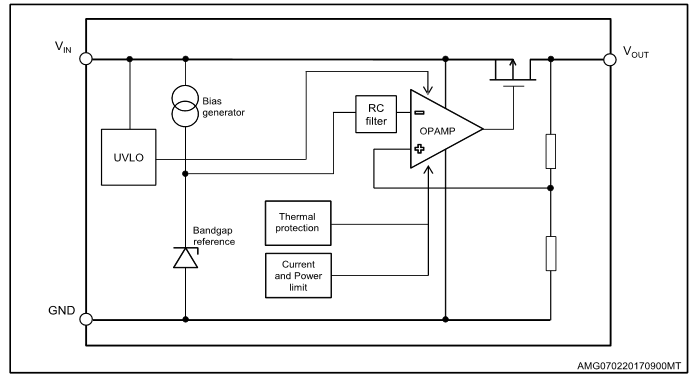
\includegraphics{Bilder/LDO.png}
	\caption{Blockschaltbild LDO}
	\label{fig:LDO}
\end{figure}

Der Differenzverstärker vergleicht die Ausgangsspannung mit einer stabilen Referenzquelle aus einer Zenerdiode, sodass diese gemessene Spannungsabweichung über das Stellglied ausgeregelt werden kann. Ist die Ausgangsspannung zu niedrig, so wird der Transistor stärker angesteuert bis die geforderte Ausgangsspannung erreicht wird, im umgekehrten Fall wird der Strom über den Transistor reduziert. Der Transistor wird in dieser Schaltung also quasi wie ein veränderlicher Widerstand verwendet, an dem die überflüssige Spannungsdifferenz abfällt. Die verwendeten LDOs besitzen außerdem eine Strombegrenzungsschaltung und eine Schutzschaltung, die die Betriebstemperatur überwacht und das Bauteil vor thermischer Überlastung schützt, sowie eine Unterspannungsabschaltung.